% Part: history
% Chapter: set-theory
% Section: limits

\documentclass[../../../include/open-logic-section]{subfiles}

\begin{document}
	
\olfileid{his}{set}{limits}	

\olsection{التعريف الصارم للنهايات}
	
الحل القياسي للمشكلة السابقة في أيامنا هو الاستغناء عن المتناهيات في
الصغر. وفيما يأتي كيفية ذلك.

رأينا أننا نحصل على تقريبات أفضل للميل كلما صغرت~$\beta$. والواقع أنه
كلما اقتربت~$\beta$ اقترابًا اعتباطيًا من~$0$، «اقترب بلا حد» مقدار
خارج قسمة الفرق
$\frac{f(c+\beta)-f(c)}{\beta}$ من الميل الذي نريده. ولذلك لا نحتاج
إلى النظر فيما يحدث \emph{عند}~$\beta = 0$؛ بل يكفينا النظر في
\emph{نزوع} خارج قسمة الفرق حين تقترب~$\beta$ من~$0$.

وبهذه الصياغة، يكون التحدي العام هو إضفاء معنى على ادعاءات من الصورة:
\begin{center}
حين تقترب~$x$ من~$c$، تقترب~$g(x)$ بلا حد من~$\ell$.
\end{center}
ويمكننا كتابة ذلك بصورة أوجز كما يأتي:
\[
\lim_{x \rightarrow c}g(x) = \ell.
\]
في القرن التاسع عشر، وبناء على أعمال سابقة لكوشي، قدم فايرشتراس
تعريفًا بالغ الصرامة لهذا التعبير. والفكرة هي فعلًا أن بوسعنا جعل
$g(x)$ قريبة من~$\ell$ بالقدر الذي نشاء، بأن نجعل~$x$ قريبة من~$c$
على نحو مناسب. وبدقة أكبر، نشترط أن تعني
$\lim_{x \rightarrow c} g(x) = \ell$ ما يأتي:
\[
(\forall\epsilon > 0)(\exists \delta > 0)\forall x \left(0 < |x-c| < \delta \lif |g(x)-\ell| < \epsilon\right).
\]
تشير الشرطتان العموديتان هنا إلى القيمة المطلقة. أي إن~$|x| = x$
حين~$x \geq 0$، و$|x| = -x$ حين~$x < 0$؛ ويمكنك رسم \emph{هذه}
الدالة كما يأتي:
\begin{center}
	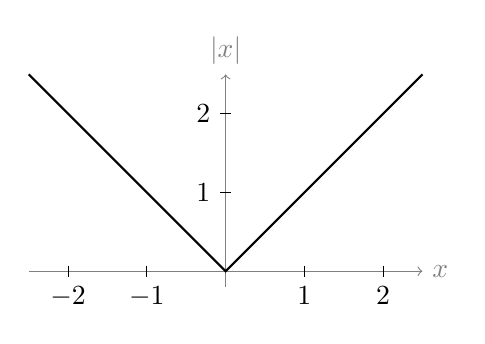
\begin{tikzpicture}[scale=1]
	\draw[->, gray] (-2.5,0) -- (2.5,0) node[right] {$x$};
	\draw[->, gray] (0,-.2) -- (0,2.5) node[above] {$|x|$};
	
	\foreach \x/\xtext in {-2/-2, -1/-1, 1/1, 2/2}
	\draw[shift={(\x,0)}] (0pt,2pt) -- (0pt,-2pt) node[below] {{$\xtext$}};
	
	\foreach \y/\ytext in {1/1, 2/2}
	\draw[shift={(0,\y)}] (2pt,0pt) -- (-2pt,0pt) node[left] {{$\ytext$}};
	
	\draw[thick] (-2.5, 2.5)--(0,0)--(2.5, 2.5);
	\end{tikzpicture}
\end{center}
ويقول التعريف، على وجه التقريب، إنك تستطيع جعل «الخطأ» أقل من
$\epsilon$ (أي~$|g(x) - \ell| < \epsilon$) باختيار مدخلات تبعد عن~$c$
مسافة أقل من~$\delta$ (أي~$|x - c| < \delta$).

وبعد تعريف مفهوم النهاية، يمكننا استخدامه للاستغناء تمامًا عن
المتناهيات في الصغر، فنشترط أن يكون ميل~$f$ عند~$c$ معطى بما يأتي:
\[
	{f}'(c) = \lim_{x \rightarrow 0}\left(\frac{f(c +x) - f(c)}{x}\right) \text{ إذا كانت النهاية موجودة}.
\]
لكن من المهم أن ندرك سبب حاجة تعريفنا إلى القيد «إذا كانت النهاية
موجودة». ولنأخذ مثالًا بسيطًا، هو~$f(x) = |x|$ التي رأينا رسمها للتو.
فمن الواضح أن~$f'(0)$ غير معرّفة تعريفًا سليمًا: إذا اقتربنا من~$0$
«من اليمين» كان الميل دائمًا~$1$؛ وإذا اقتربنا من~$0$ «من اليسار» كان
الميل دائمًا~$-1$؛ ولذلك لا تكون النهاية معرّفة. ومن ثم يمكن أن نضيف
أن الدالة~$f$ تكون \emph{قابلة للاشتقاق} عند~$x$ إذا وفقط إذا كانت
هذه النهاية موجودة.

رأينا كيف نعالج الاشتقاق باستخدام مفهوم \emph{النهاية}. ويمكننا
استخدام المفهوم نفسه لتعريف الدالة \emph{المتصلة}. (وكان بولتسانو قد
أدرك ذلك بالفعل بحلول عام 1817.) وتعالج طريقة كوشي--فايرشتراس الاتصال
على النحو الآتي. على وجه التقريب، تكون الدالة~$f$ متصلة عند نقطة إذا
كان في وسعك، متى طلبت مقدارًا معينًا من الدقة في مخرج الدالة، أن تضمن
ذلك باشتراط مقدار معين من الدقة في مدخلها. وبدقة أكبر، تكون~$f$ متصلة
عند~$c$ إذا كان الفرق بين~$f(c + x)$ و$f(c)$ نفسها يقترب من~$0$ حين
تقترب~$x$ من الصفر. وبعبارة أخرى، تكون~$f$ \emph{متصلة} عند~$c$ إذا
وفقط إذا كان~$f(c) = \lim_{x \rightarrow c} f(x)$.

لن يقودنا التوغل أبعد من ذلك إلا إلى التحليل الحقيقي، في حين أن
موضوعنا هو نظرية المجموعات. فلنتوقف الآن ونبين المغزى. تعلم الرياضيون
خلال القرن التاسع عشر كيف يستغنون عن المتناهيات في الصغر باستدعاء
مفهوم \emph{النهاية} المعرّف تعريفًا صارمًا.

\end{document}
